\documentclass[12pt, english, letter]{article}


\usepackage[T1]{fontenc}
\usepackage{babel}

\usepackage{braket}
\usepackage{url}

\usepackage{graphicx}
\usepackage{epstopdf}
\usepackage[labelfont=sf,it,bf , textfont=sf, format=plain]{caption}

\usepackage[backend=biber, style=chem-angew, autocite=superscript,]{biblatex}
\addbibresource{nature.bib}


\title{Supporting Information: \\ Identifying Free Energy Hot-Spots\\ in Molecular Transformations}

\author
{Johannes C. B. Dietschreit,$^{1,2}$ Laurens D. M. Peters,$^{1,2}$\\ J\"org Kussmann$^{1,2}$, Christian Ochsenfeld$^{1,2}$\\
	\\
	\normalsize{$^{1}$Center for Integrated Protein Science (CIPSM) at the Department of Chemistry,}\\
	\normalsize{University of Munich (LMU), Butenandtstr.~5--13, D-81377 M\"unchen, Germany}\\
	%
	\normalsize{$^{2}$Chair of Theoretical Chemistry,  Department of Chemistry,}\\
	\normalsize{University of Munich (LMU), Butenandtstr.~7, D-81377 M\"unchen, Germany}\\
}
% Include the date command, but leave its argument blank.

\date{}



\newcommand{\aglu}{\textbf{$\alpha$-Glu}}
\newcommand{\bglu}{\textbf{$\beta$-Glu}}
\newcommand{\ahct}{\textbf{$\alpha$-HCT}}
\newcommand{\bhct}{\textbf{$\beta$-HCT}}
\newcommand{\bet}{\textbf{BET}}
\newcommand{\agluahct}{\textbf{I}}
\newcommand{\bglubhct}{\textbf{II}}
\newcommand{\aglubglu}{\textbf{III}}
\newcommand{\ahctbhct}{\textbf{IV}}
\newcommand{\avib}{A_\mathrm{vib}}

\renewcommand{\theequation}{S\arabic{equation}}

\begin{document}
	
	\maketitle
	
	\renewcommand\figurename{SFigure}
	%\setcounter{figure}{0}
	%\renewcommand\pagemark{S\thepage}
	%\setcounter{page}{1}
	
	
%	{\sffamily \textbf{Table of Contents}}
%	\begin{itemize}
%		\item Materials and Methods
%		\begin{itemize}
%			\item Quantum Mechanics Simulations
%			\item Classical Mechanics Simulations
%			\item Free Energy Calculations
%			\item Infrared Spectra
%			\item Image Processing
%		\end{itemize}
%		\item Data and Material Availability
%		\item Figures S1 to S4
%	\end{itemize}
%	\vspace{2cm}

\tableofcontents
	
	%\small
	\section{Materials and Methods}
	
	\subsection{Quantum Mechanics Simulations}
	
	The quantum chemistry package \emph{FermiONs++}\autocite{Kussmann2013,Kussmann2015} developed in our group was used for the \textit{ab initio} Born-Oppenheimer molecular dynamics simulations. We used the HF-3c\autocite{Sure2013} method that includes dispersion (DFTD3 v3.1)\autocite{Grimme2010,Grimme2011} and counterpoise corrections (gCP v2.02)\autocite{Kruse2012}. The Velocity Verlet algorithm\autocite{Verlet1967,Swope1982} and a stochastic rescaling thermostat\autocite{Bussi2007} were applied. The structures of \aglu{}, \bglu{}, \ahct{}, and \bhct{} were minimized at the same level of theory before the calculations. The initial atom velocities were drawn at random from a Maxwell-Boltzmann distribution at 298.15~K. The time step was 0.5~fs and a 9th order extended Lagrangian scheme\autocite{Niklasson2009} was used to improve the SCF convergence. The system was equilibrated for 5~ps. The production runs were 200~ps long and 20 independent simulations were conducted for each molecule. Translation and rotation of the molecule were removed at every step of the simulation. As starting points we used the global as well as local minima to enhance the sampling of the phase space.
	
	\subsection{Classical Mechanics Simulations}
	
	The crystal structures of the apo-bromodomain (PDB 5O38)\autocite{Runcie2018} and the inhibitor-domain complex (PDB 5O3B)\autocite{Runcie2018} were used as starting structures. All molecules that were not protein, inhibitor, or water were removed. Antechamber, part of the AmberTools 16\autocite{Case2017}, was used to parametrize the inhibitor. The force field ff14SB\autocite{Maier2015} was used for the simulations. The proteins were solvated in a rectangular box with 10~Angstrom of TIP3P\autocite{Jorgensen1983} water, and neutralized with 2 chlorine ions. The simulation engine NAMD\autocite{Phillips2005} was used. The system was minimized, for the first 10,000 steps only the water molecules and for the next 10,000 steps the full system. The system was heated over 30~ps to 300~K. In the following it was equilibrated for 200~ps and then production runs of 1~ns were carried out. The time step was 0.5~fs. Non-bonded interactions were evaluated at every step. Periodic electrostatic interactions were computed with the particle mesh Ewald summation method, with a 6$^\mathrm{th}$ order interpolation. We used a cut-off radius of 12~\AA\, and a switching function that smoothly switched off interaction between 10 and 12~\AA. A Verlet nearest neighbour list with a radius of 13.5~\AA\, was used. The temperature was controlled with the Berendsen rescaling algorithm\autocite{Berendsen1984}. Coordinates and velocities were written to file every 1~fs. Translation and rotation of the protein were removed from the velocities after the simulation. \emph{MDAnalysis} \autocite{MDAnalysis1, MDAnalysis2} was used to extract and process the velocities.
	
	\subsection{Free Energy Calculations}
	
	Total free energies ($A$) are calculated from the sampled nuclear velocities applying Eqs.~(1) and (2). All atomic spectra were rescaled such that every atom received the same fraction of the total amount of degrees of freedom. Their two contributions, the potential energy at the minimum energy geometry ($E$) and the vibrational free energy ($\avib$), cover static and dynamic changes, respectively. Free energies from rotation and translation can often be neglected, as (1) their contributions are often distributed over the entire molecule and generally small (when free energy differences ($\Delta A$) are considered) and (2) the overall rotation and translation of the system are removed at every step of the simulation (see previous section), because keeping them can lead to unwanted artefacts. $D(\nu)$ is, therefore, the vibrational density of state function or the vibrational power spectrum. Please note that, when calculating energy differences of single molecules and not ensembles, $\Delta A$ is equivalent to the change of the Gibbs free energy ($\Delta G$), as pressure and volume do not contribute. In order to obtain atom- or residue-resolved free energies, we recast Eq.~(1) to
	
	\begin{eqnarray}
	D(\nu) & = & 2 \beta \sum \limits_{j = 1}^{N} m_j \int dt
	\braket{\mathbf{v}_j (\tau) \mathbf{v}_j (t + \tau)}_{\tau} e^{-i 2\pi \nu t} \nonumber \\
	& = & \sum \limits_{j = 1}^{N} 2 \beta m_j \int dt
	\braket{\mathbf{v}_j (\tau) \mathbf{v}_j (t + \tau)}_{\tau} e^{-i 2\pi \nu t} \nonumber \\ 
	& = & \sum \limits_{j = 1}^{N} D_j(\nu) \nonumber \\ 
	& = & \sum \limits_{i}^{N_\mathrm{regions}} \sum \limits_{j}^{\{N\}_i} D_j(\nu).
	\end{eqnarray}
	%
	$N_\mathrm{regions}$ is the number regions in which we split the total system and $\{N\}_i$ is the set of atoms that belong to the region $i$. The regions can be chosen completely freely ranging from the entire system to individual atoms.  This helps us rewrite Eq.~(2) to
	%
	\begin{eqnarray}
	A & = E + \sum \limits_{i}^{N_\mathrm{regions}} \avib{}(i).
	\end{eqnarray}
	%
	$\avib{}(i)$ is the vibrational free energy localized in region $i$. If we consider free energy changes
	%
	\begin{eqnarray}
	\Delta A & = \Delta E + \sum \limits_{i}^{N_\mathrm{regions}} \Delta  \avib{}(i),
	\end{eqnarray}
	%
	$\Delta  \avib{}(i)$ indicates a change in the potential energy surface in region $i$ and it can be safely assumed that $\Delta E$ is influenced only by those regions of the potential energy surface which are changing. Thus, the local changes in $\avib{}$ serves as an indicator for affected parts of the system. 

	
	\section{Infrared Spectra}
	
	The experimental spectrum of D(+)-glucose 1-hydrate (ITW Reagents, $>$99\%) has been measured in this work as an average of 16 scans with 1 cm$^{-1}$ resolution using a Thermo Fischer Nicolet 6700 FT-IR apparatus.
	
	\section{Image Processing}
	
	All images containing molecular geometries which are coloured according to changes in vibrational free energy were produced using \emph{VMD}\autocite{HUMP96}. All plots showing spectra and distributions were produced using the python-package \emph{matplotlib}\autocite{Hunter2007}. The chemical structures were drawn with \emph{ChemDraw}.
	
	\section{Data and Materials Availability}
	%
	All inputs and trajectories are available upon request. PDB files (with the free energy colouring), analysis scripts, and an interactive tutorial are available at \url{http://www.cup.lmu.de/pc/ochsenfeld/download/}. \emph{NAMD} is freely available for non-commercial users, while \emph{FermiONs++} is not yet available. 
	
	\newpage
	
	\section{Figures}
	
	\begin{figure}[h!]
		\centering
		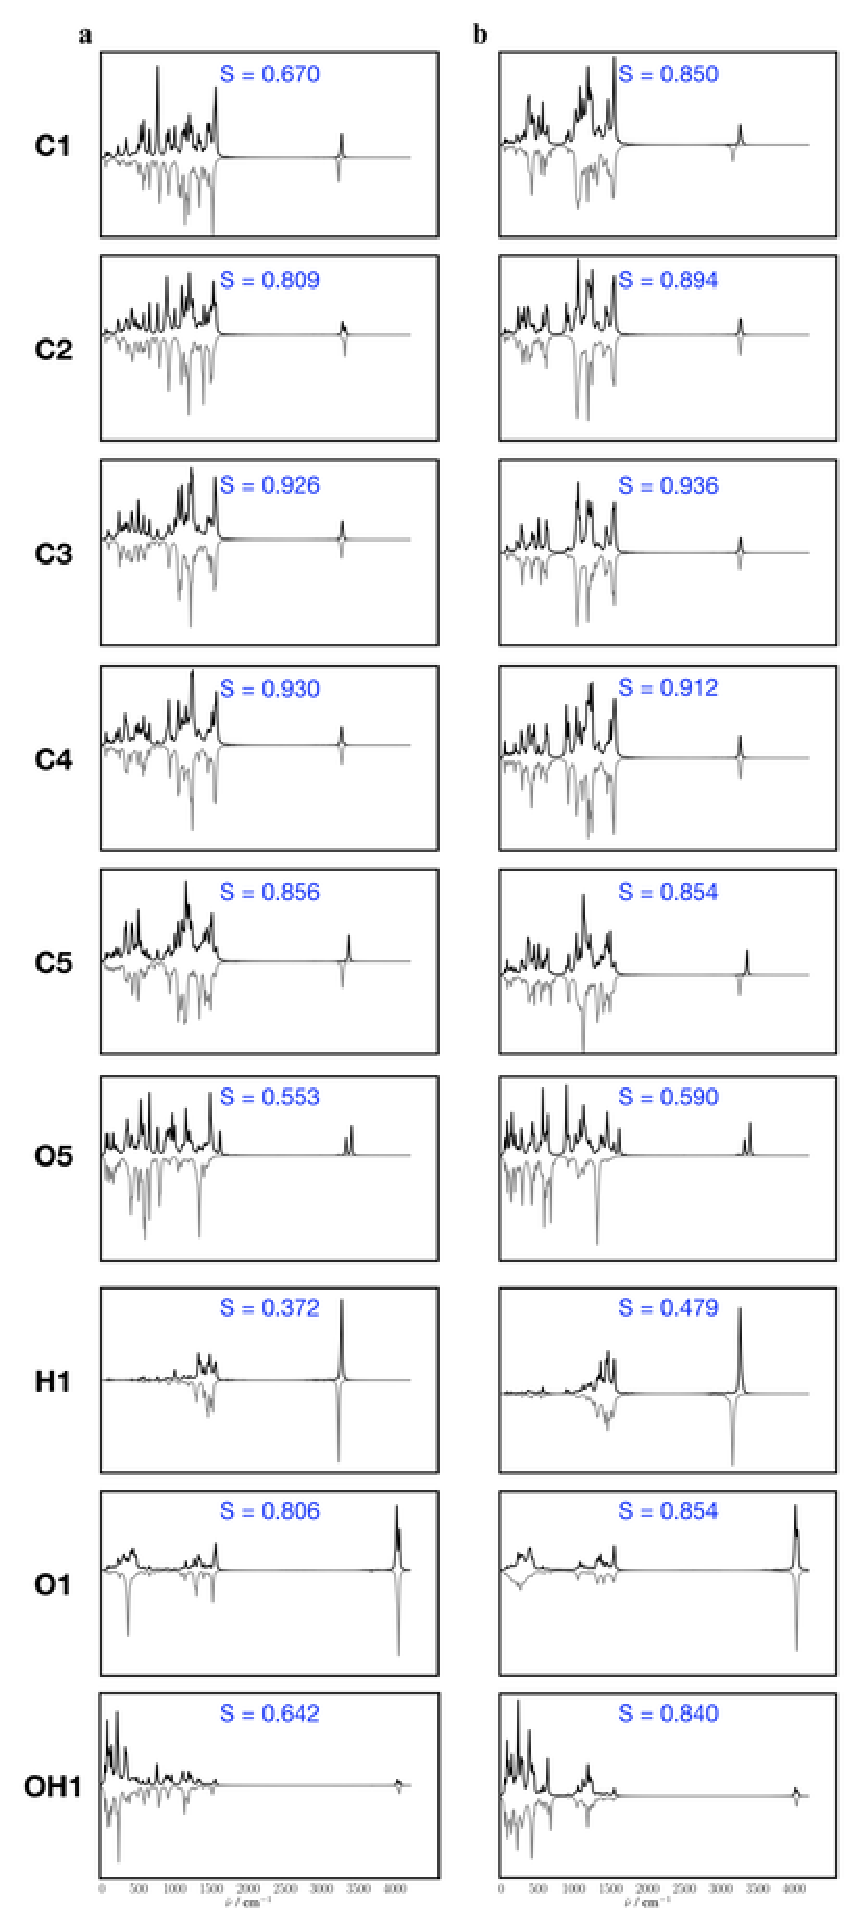
\includegraphics[height=0.7\textheight]{sfig1.eps}
		\caption{%\textbf{Vibrational spectra and overlaps}.
			\textbf{a}+\textbf{b}, Vibrational spectra per atom for (\textbf{a}) \ahct{} (black) and \aglu{} (inverted grey) and (\textbf{b}) \bhct{} (black) and \bglu{} (inverted grey). The overlap ($S$) between the two spectra is calculated as 
			$	
			S = \int_0^\infty I_1(\tilde{\nu}) I_2(\tilde{\nu}) \mathrm{d} \tilde{\nu} /
			\sqrt{\int_0^\infty I_1^2(\tilde{\nu}) \mathrm{d} \tilde{\nu} \int_0^\infty I_2^2(\tilde{\nu}) \mathrm{d}  		\tilde{\nu}} ,
			$
			with $I_1$ and $I_2$ being the intensity of the two spectra at a wavenumber ($\tilde{\nu})$). The overlap between \aglu{} and \ahct{} is generally smaller than the overlap between \bglu{} and \bhct{}. The wave number ($\tilde{\nu}$) increases from left to right.
		}
		\label{fig:glucose_appendix}
	\end{figure}
	
	\newpage
	
	\begin{figure}[h!]
		\centering
		\includegraphics[width=0.9\textwidth]{sfig2.eps}
		\caption{%\textbf{Coordinate-based signs of the anomeric effect.} 
			Distribution of bond lengths and angles of the simulations of (left column) \aglu{} and \bglu{} and (right column) \ahct{} and \bhct{}, that serve as an indicator for the anomeric effect. \aglu{} exhibits, in comparison to \bglu{}, a shorter C1-O5 bond, a longer C1-O1 and C5-O5 bond, and a smaller C5-O5-C1-C2 dihedral angle. Similar observations cannot be made, when comparing the simulations of \ahct{} and \bhct{}.}
		\label{fig:glucose_distr}
	\end{figure}
	
	\newpage
	
	\begin{figure}[h!]
		\centering
		\includegraphics[width=1.0\textwidth]{sfig3.eps}
		\caption{%\textbf{Comparison of vibrational IR- and power-spectrum}.
			(Top) Experimental IR spectrum of crystalline glucose-mono-hydrate (black) and simulated IR spectra (calculated as presented in \autocite{Peters2017}) of \aglu{} (orange) and \bglu{} (blue). (Bottom) Computed vibrational power spectra of \aglu{} (orange) and \bglu{} (blue). The power spectrum has different intensities and also shows not IR-active vibrations exhibiting a small or no change in the dipole moment. For comparison to the experiment, the simulated spectra have been scaled by a factor of $0.82$ (similar to the reported $0.81$\autocite{Peters2017}).
		}
		\label{fig:ir_vs_pow}
	\end{figure}
	
	\newpage
	
	\begin{figure}[h!]
		\centering
		\includegraphics[width=0.95\textwidth]{sfig4.eps}
		\caption{%\textbf{Vibrations affected by the anomeric effect}.
			Other vibrations than the C-H stretching bond are affected by the anomeric effect, e.g., the C-H deformation mode, which is clearly shifted in the case of \aglu{}. For comparison to the experiment, the simulated spectra have been scaled by a factor of $0.82$ (similar to the reported $0.81$\autocite{Peters2017}).
		}
		\label{fig:c1_vibration}
	\end{figure}

\newpage

\printbibliography[heading=bibintoc]


\end{document}